%%%%%%%%%%%%%%%%%%%%%%%%%%%%%%%%%%%%%%%%%%%%%%%%%%%%%%%%%%
\section{Introduction}
%%%%%%%%%%%%%%%%%%%%%%%%%%%%%%%%%%%%%%%%%%%%%%%%%%%%%%%%%%

The human fovea provides a small window of high acuity vision to the world, and the locations that we select to view through this window can tell us how we seek the information necessary to complete the task we are currently undertaking. Fixation locations are selected based on a combination of low-level factors such as visual salience \citep{borji2013} and high-level factors \citep{yarbus1967, buswell1935, land2001}. However, there are also strong observable biases in eye movements that are independent of the content of the scene or the task being performed \citep{tatler-vincent2009, foulsham2010}, such as a strong tendency to fixate near to the centre of images \citep{tatler2007, canosa2003, stainer2013}. If we are to gain a complete understanding of the factors that govern how we sample information, we must build models of eye guidance on the framework of these underlying biases, using them as a baseline against which to compare effects of the scene, task, image properties and individual differences.

%%%%%%%%%%%%%%%%%%%%%%%%%%%%%%%%%%%%%%%%%%%%%%%%%%%%%%%%%%%%%
\subsection{Eye movement heuristics}
%%%%%%%%%%%%%%%%%%%%%%%%%%%%%%%%%%%%%%%%%%%%%%%%%%%%%%%%%%%%%

One influential model of eye movements of the last decade is the optimal search model \citep{najemnik-geisler2008}, which posits that human saccadic behaviour during visual search is consistent with predictions made by an ideal observer. The number of fixations human observers needed to make to find the target was closely matched by the ideal observer model, in which successive fixations were selected based on reducing uncertainty about the target's location, taking into account search history and target visibility across the visual field. The efficiency of human search (at least, in search for a Gabor patch hidden in $1/f$-noise) suggests this as a plausible mechanism for selecting fixations during search. Further evidence for this theory comes from \cite{ma2011} who found that human observers are near-optimal in a visual search task with line segments, and presented a neural network implementation of near-optimal search based on probabilistic population coding.  

While this modelling framework is attractive, there are several issues. The computations driving each fixation are complex, and depend on a fairly precise representation of one's own acuity over the visual field for a wide range of possible target/background combinations. One might therefore question the assumption that these computations are undertaken to determine the location of each of the 3-4 fixations made on average every second during visual search. More importantly,  \cite{morvan-maloney2012} demonstrated that human observers are not able to use information about visual sensitivity in the periphery to rationally plan even a single saccade to the optimal location in a target discrimination task. In their experiment, the observer simply has to select a location from which to detect a target that can appear with equal probability in one of two possible locations. If the locations are relatively close together, a location in between will maximise the probability of detecting a target appearing in either location. When the targets are too far apart to reliably detect the target from a point equidistant between them, the rational strategy is to look directly at one of the two possible target locations. Inconsistent with optimal viewing strategies, however, the observers did not systematically modify their choice about where to fixate according to the distance between the possible target locations. This striking failure of optimality has recently been replicated in a larger sample and generalised to other decisions in addition to eye movements  \citep{clarke-hunt2015}. To reconcile their results with those of  \cite{najemnik-geisler2008},  \cite{morvan-maloney2012} suggest \textit{heuristics} guide saccade planning; that is, basic oculomotor biases such as a tendency to make saccades of particular amplitudes, and/or to particular regions of a display, or in particular sequences, depending on the current task. 

This idea has recently been formalised in a model by \cite{clarke2016}, who demonstrate that a stochastic search model based on a memoryless random walk can find a target in noise in a similar number of fixations to human observers. The key component of this model was the use of the empirical distribution of saccades: for each saccade the model randomly samples a saccade from distributions estimating the likelihood a human observer made a saccade from $(x_{i+1},y_{i+1})$ to $(x_i,y_i)$. It is clear from Figure \ref{fig:empiricalSaccadicFlow} that the distribution of saccade end points varies considerably depending on where the saccade is launched from. Thus a model that accounts for these launch-site dependent differences in exploration biases has the potential to offer a better account of viewing behaviour. This stochastic model differs from the random baseline implemented by \cite{najemnik-geisler2008}, in which they randomly selected each fixation location from all possible points in the display, because it incorporates basic oculomotor heuristics that guide the eyes, without the need for complex computation of peripheral sensitivity or target location probability. 

This stochastic search model is related to the more general topic of saccadic biases. Recent work in this area by \cite{leMeur-coutrot2016} independently arrived at a very similar model to \cite{clarke2016} while investigating context-dependent and spatially-variant veiwing biases. Both their model and the Stochastic Search model partitioned the data into $k\times k$ subsets (\cite{leMeur-coutrot2016} used $k=3$ while \cite{clarke2016} used $k=5$) and then used non-parametric methods to model the distributions. In this paper, we re-implement and generalise this idea with a parameter named \textit{Saccadic Flow}, and examine the extent to which it is useful as a prior for analysing eye movements made with more natural (photographic) stimuli over a range of different tasks. 


\begin{figure}[htb]
\centering
\subfigure{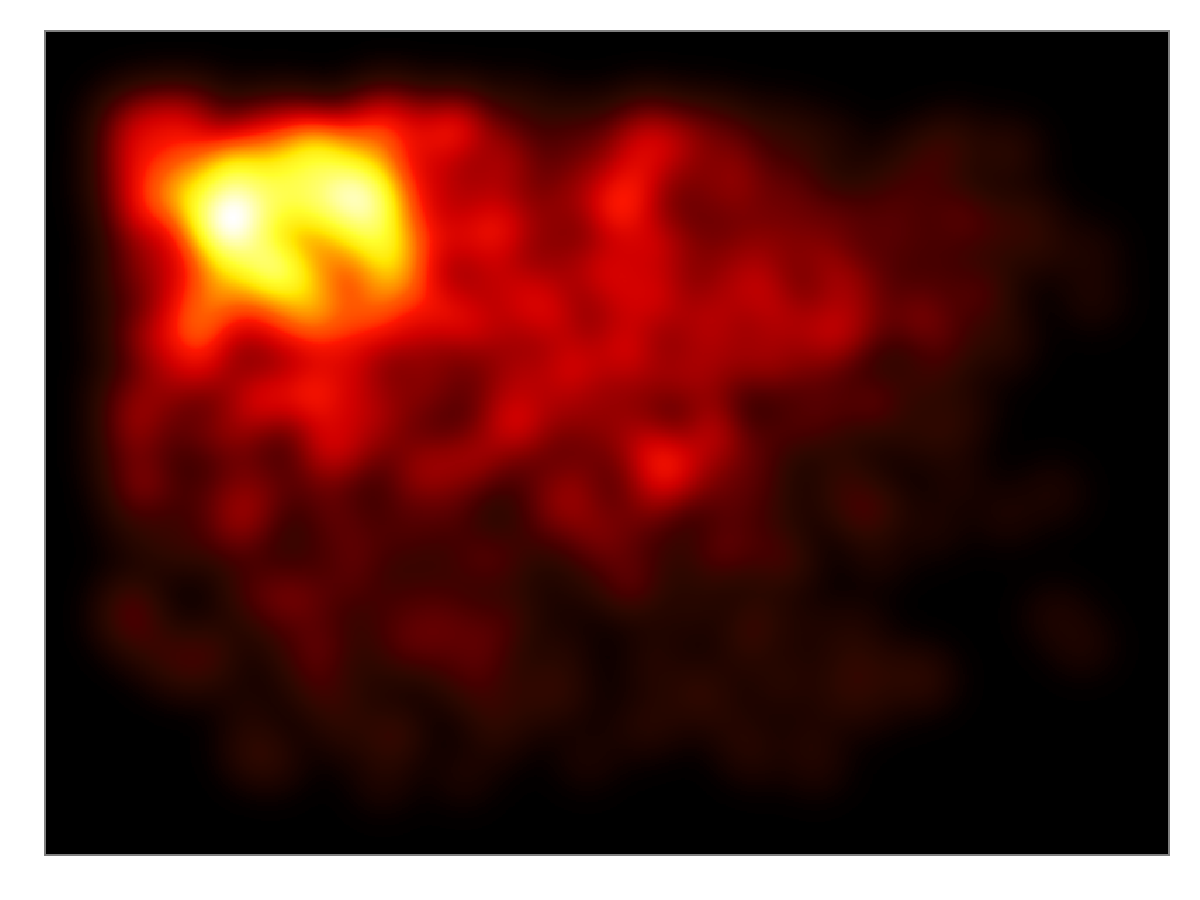
\includegraphics[width=2.5cm]{../scripts/heatmaps/SaccadicFlowMaps/Figures/BBias_11.pdf}}
\subfigure{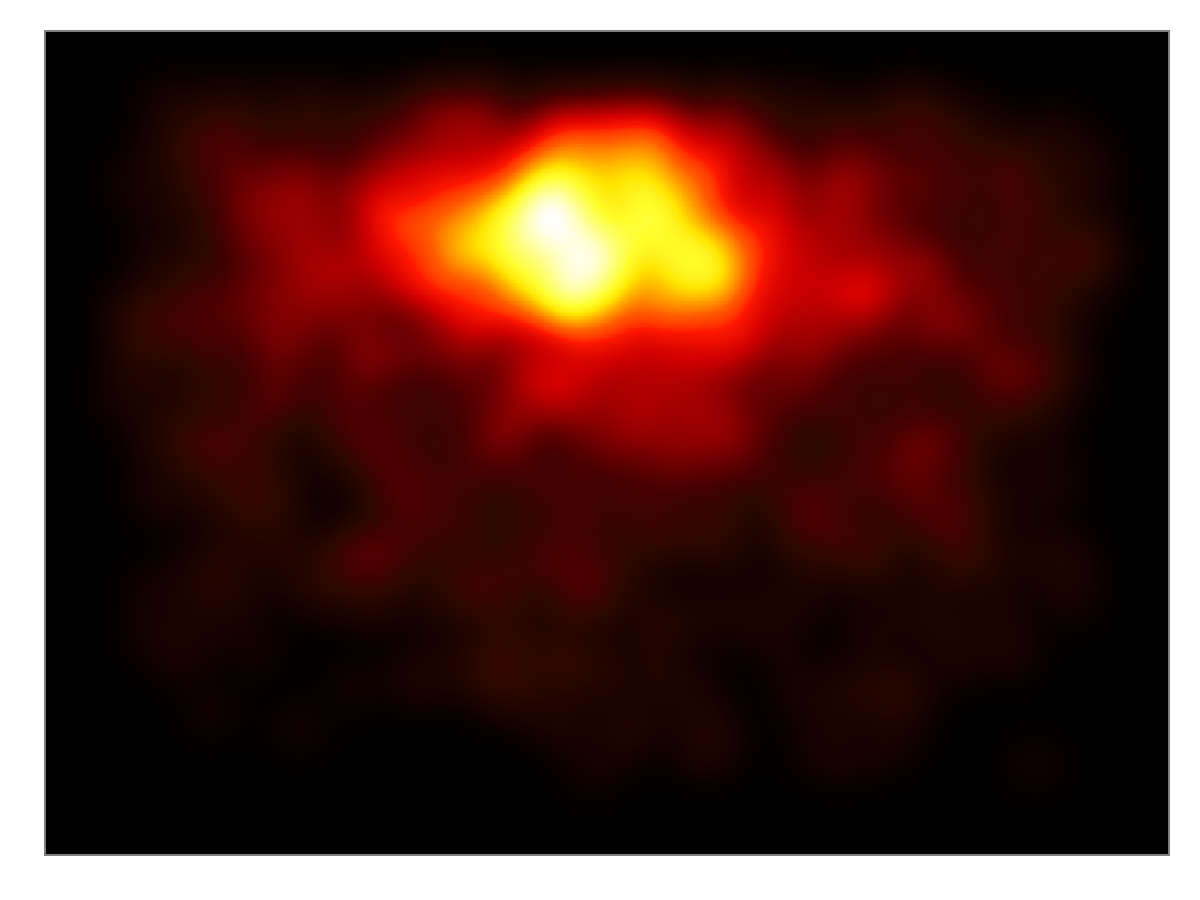
\includegraphics[width=2.5cm]{../scripts/heatmaps/SaccadicFlowMaps/Figures/BBias_12.pdf}}
\subfigure{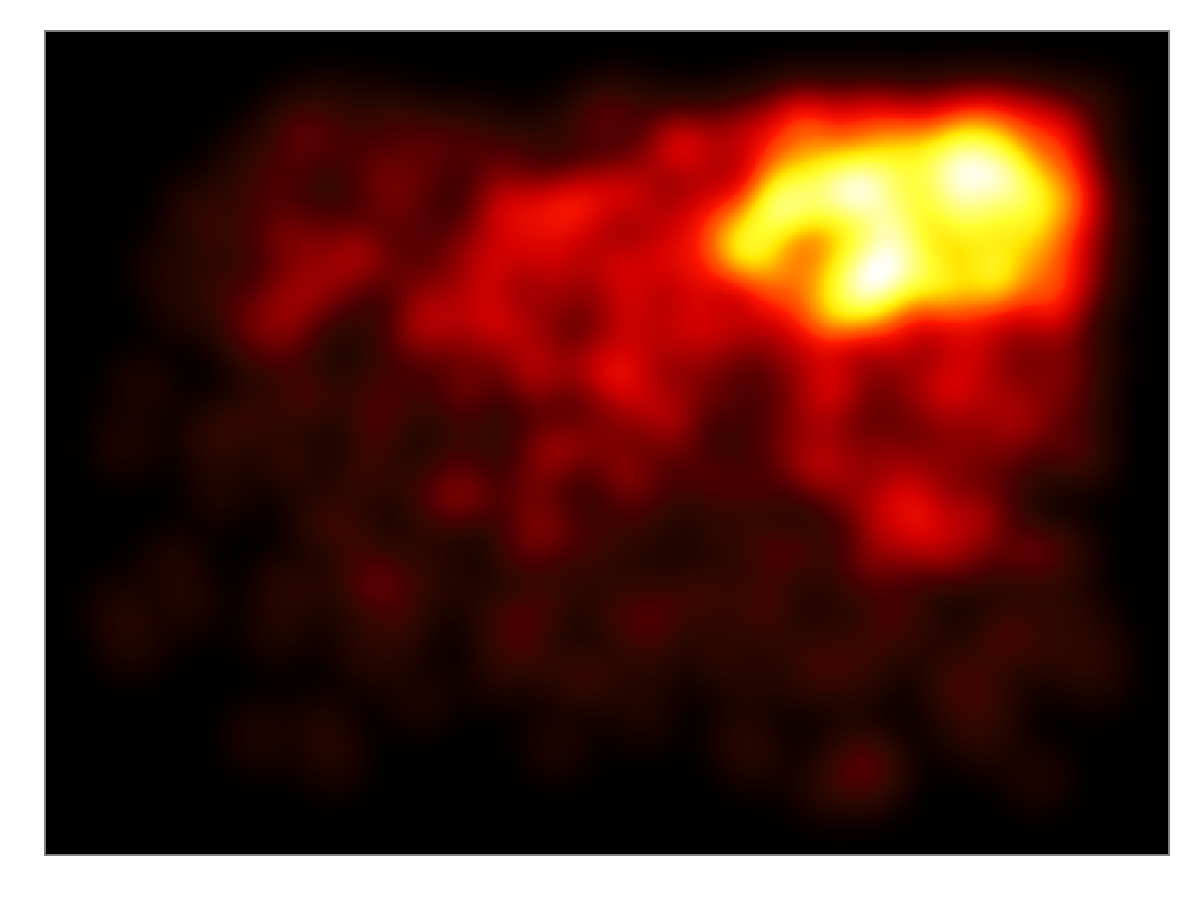
\includegraphics[width=2.5cm]{../scripts/heatmaps/SaccadicFlowMaps/Figures/BBias_13.pdf}}
\subfigure{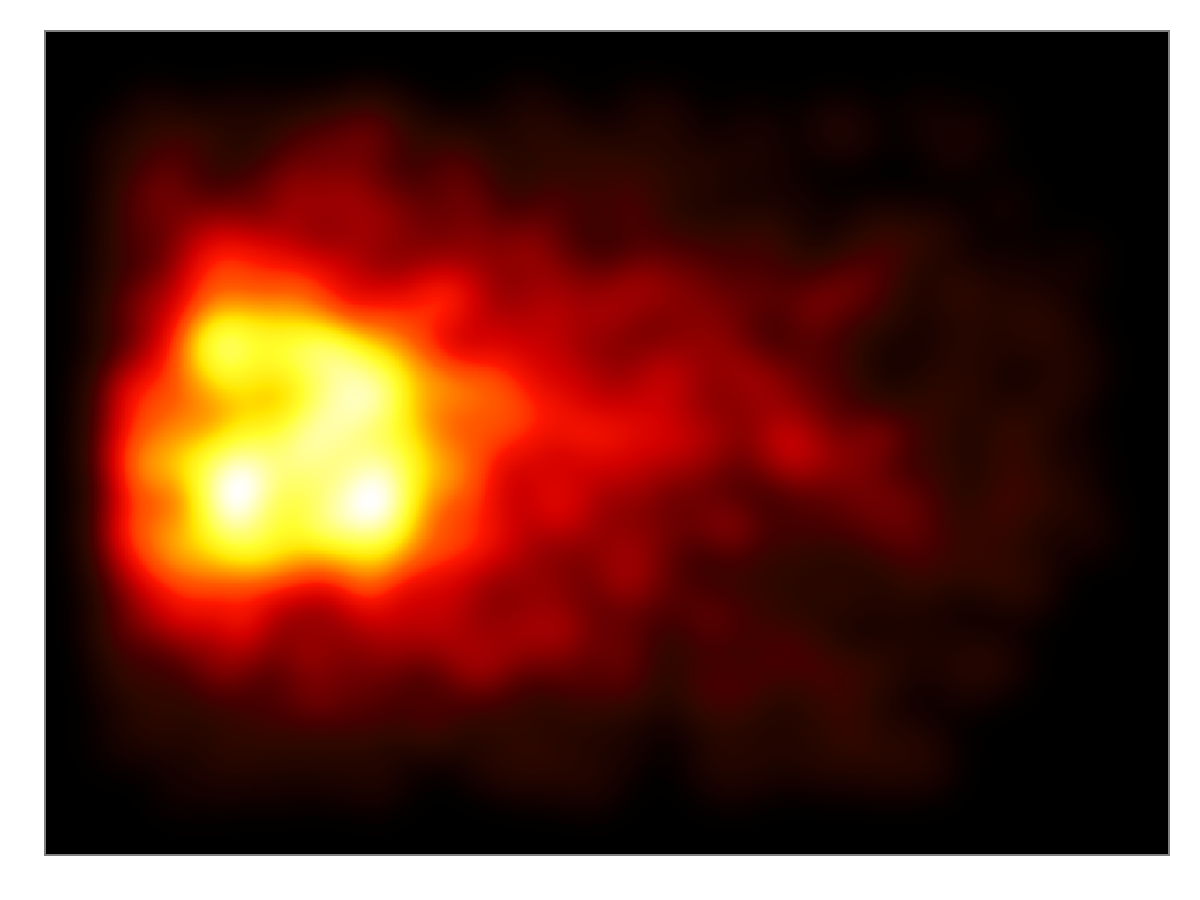
\includegraphics[width=2.5cm]{../scripts/heatmaps/SaccadicFlowMaps/Figures/BBias_21.pdf}}
\subfigure{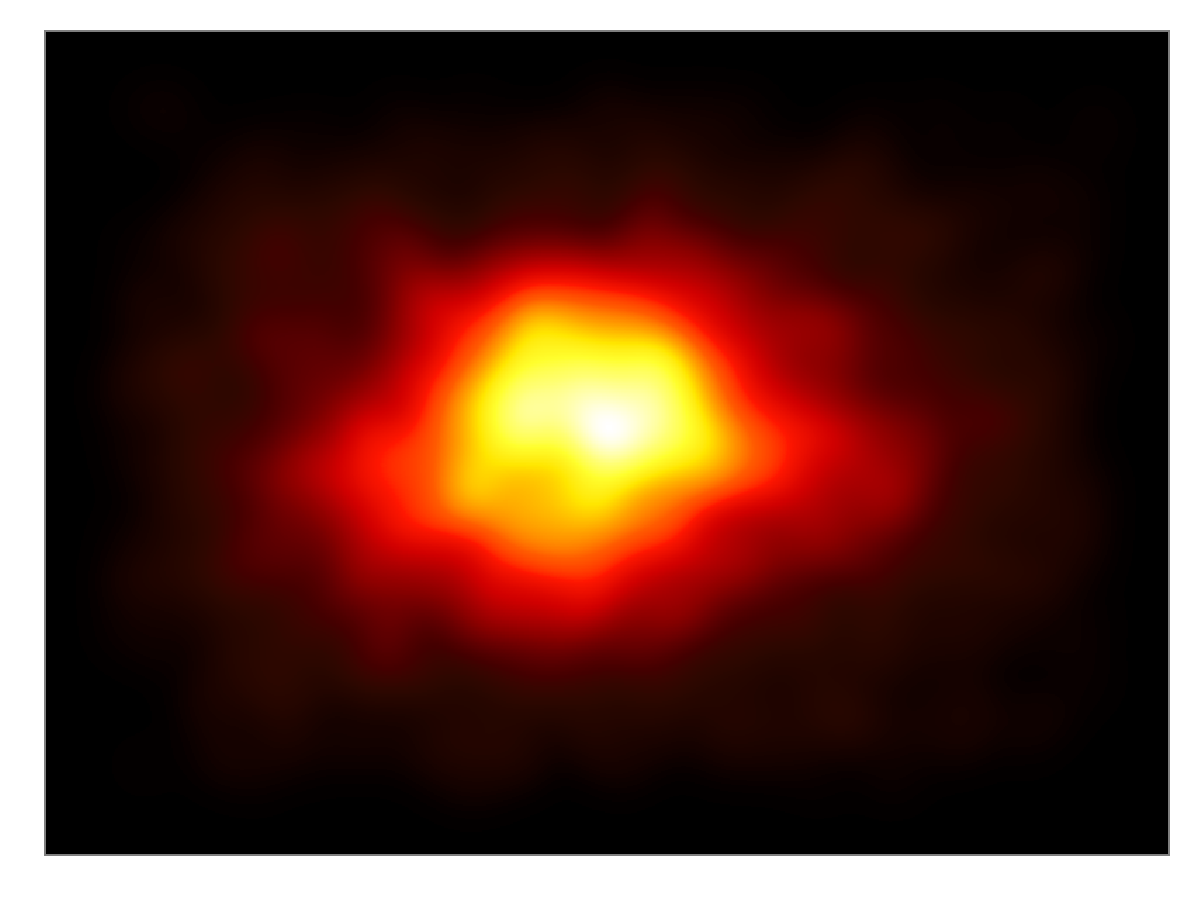
\includegraphics[width=2.5cm]{../scripts/heatmaps/SaccadicFlowMaps/Figures/BBias_22.pdf}}
\subfigure{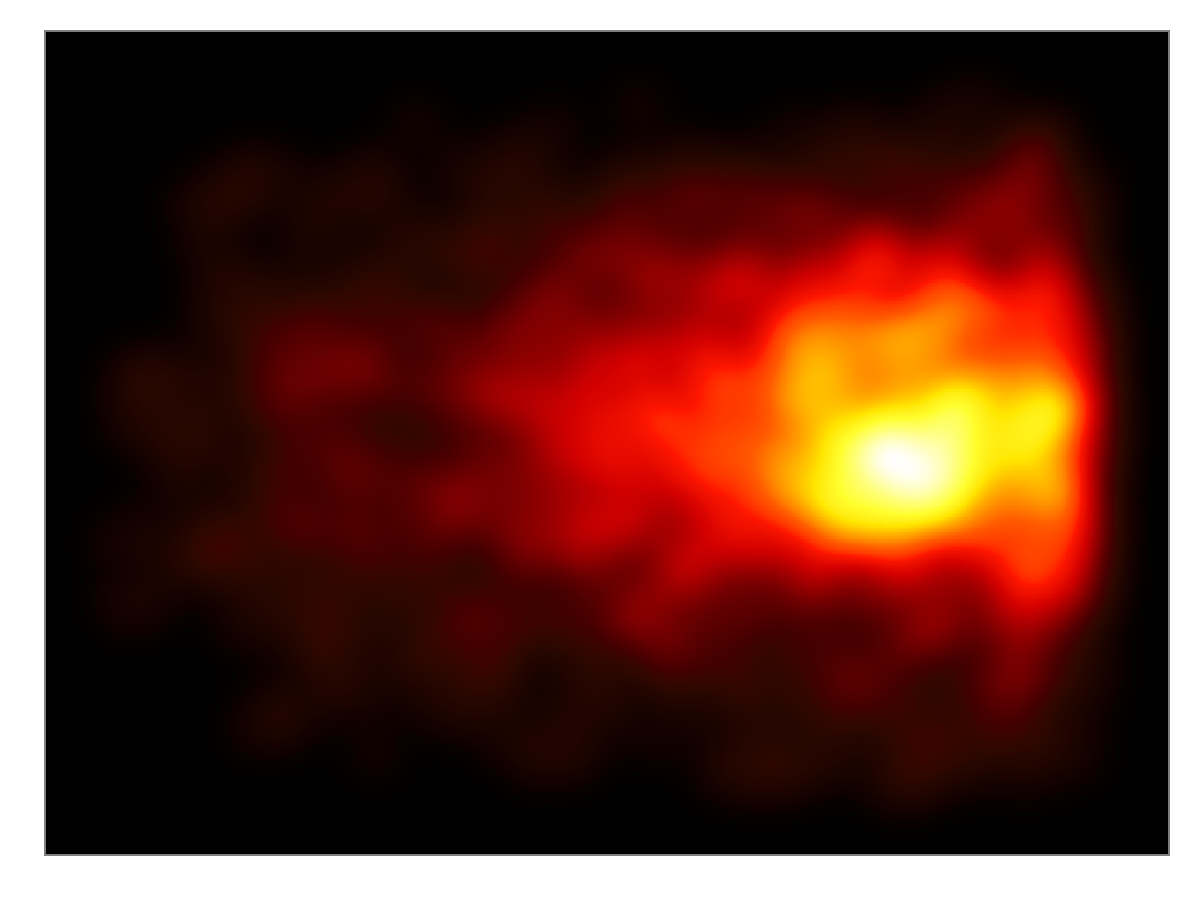
\includegraphics[width=2.5cm]{../scripts/heatmaps/SaccadicFlowMaps/Figures/BBias_23.pdf}}
\subfigure{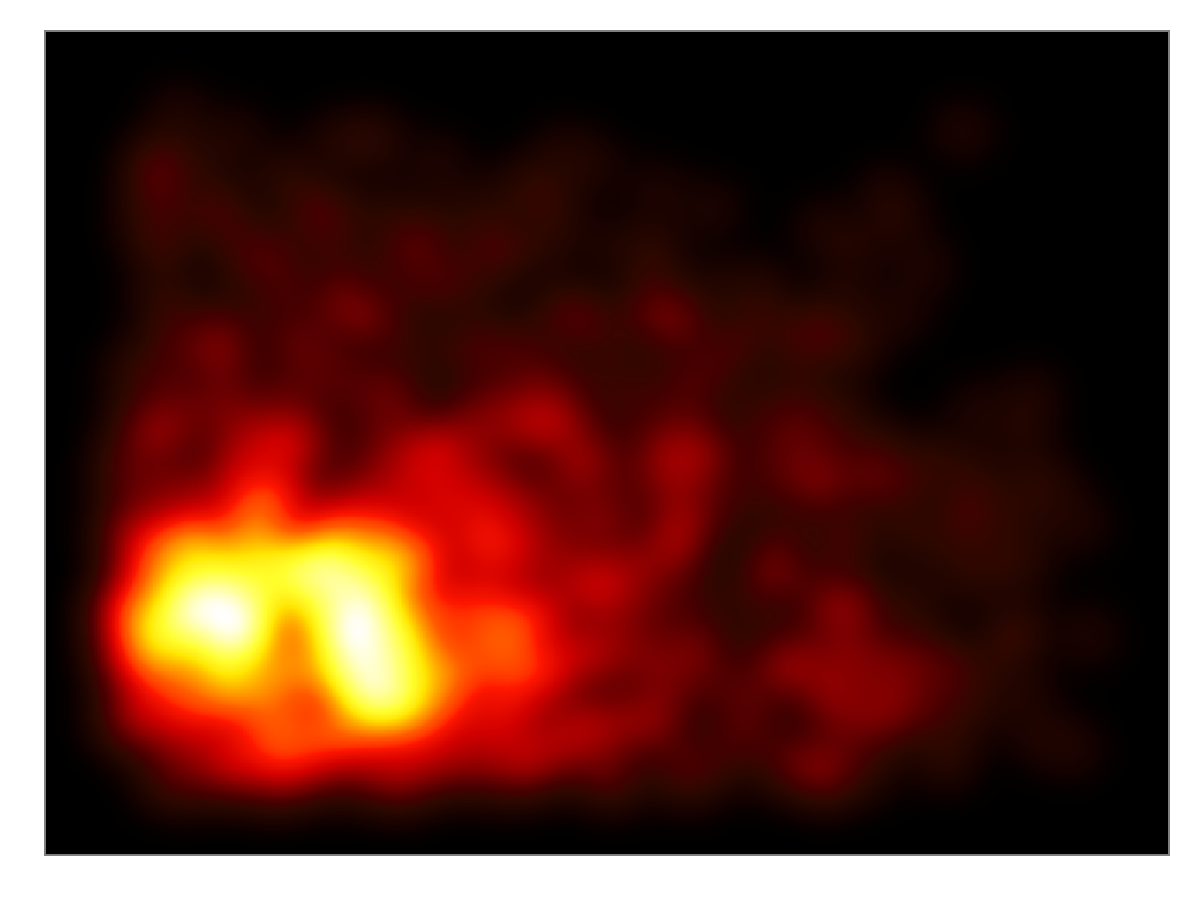
\includegraphics[width=2.5cm]{../scripts/heatmaps/SaccadicFlowMaps/Figures/BBias_31.pdf}}
\subfigure{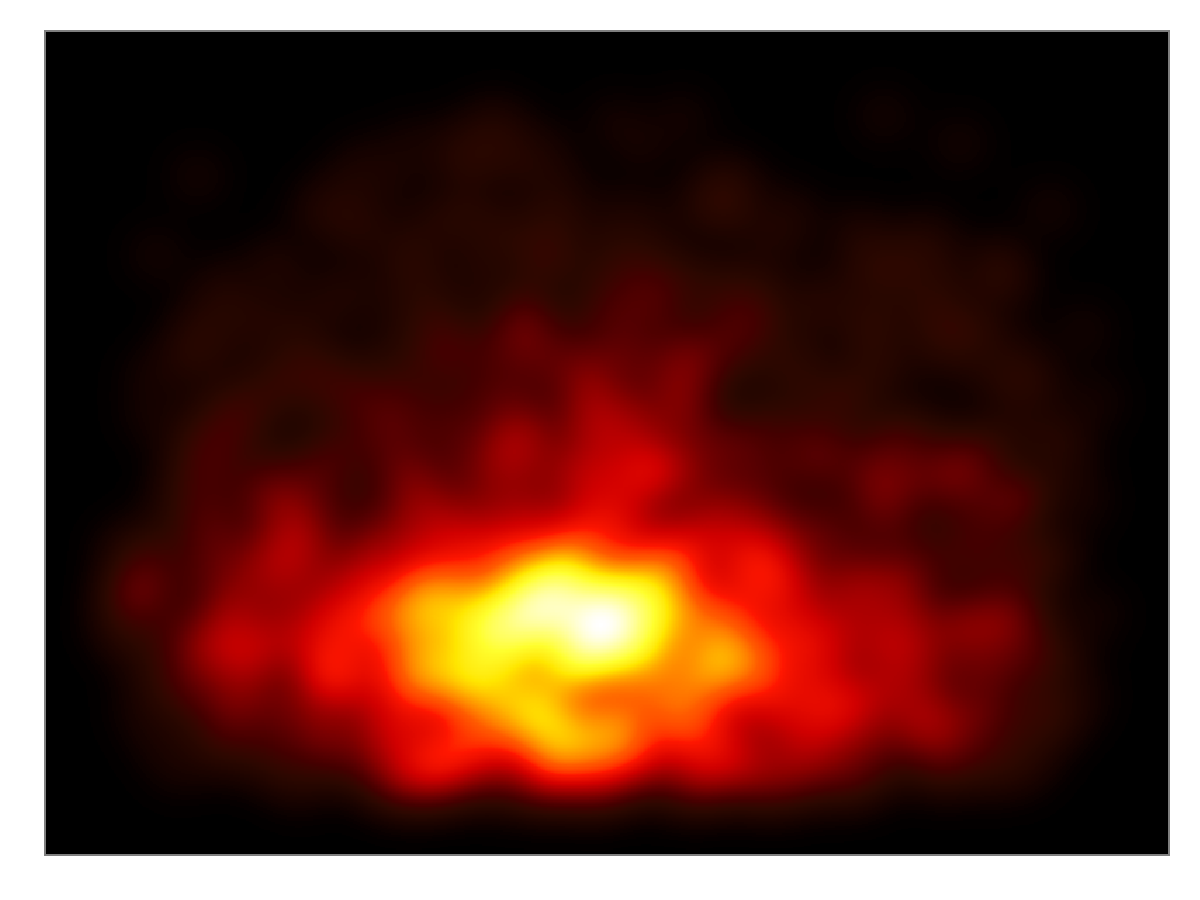
\includegraphics[width=2.5cm]{../scripts/heatmaps/SaccadicFlowMaps/Figures/BBias_32.pdf}}
\subfigure{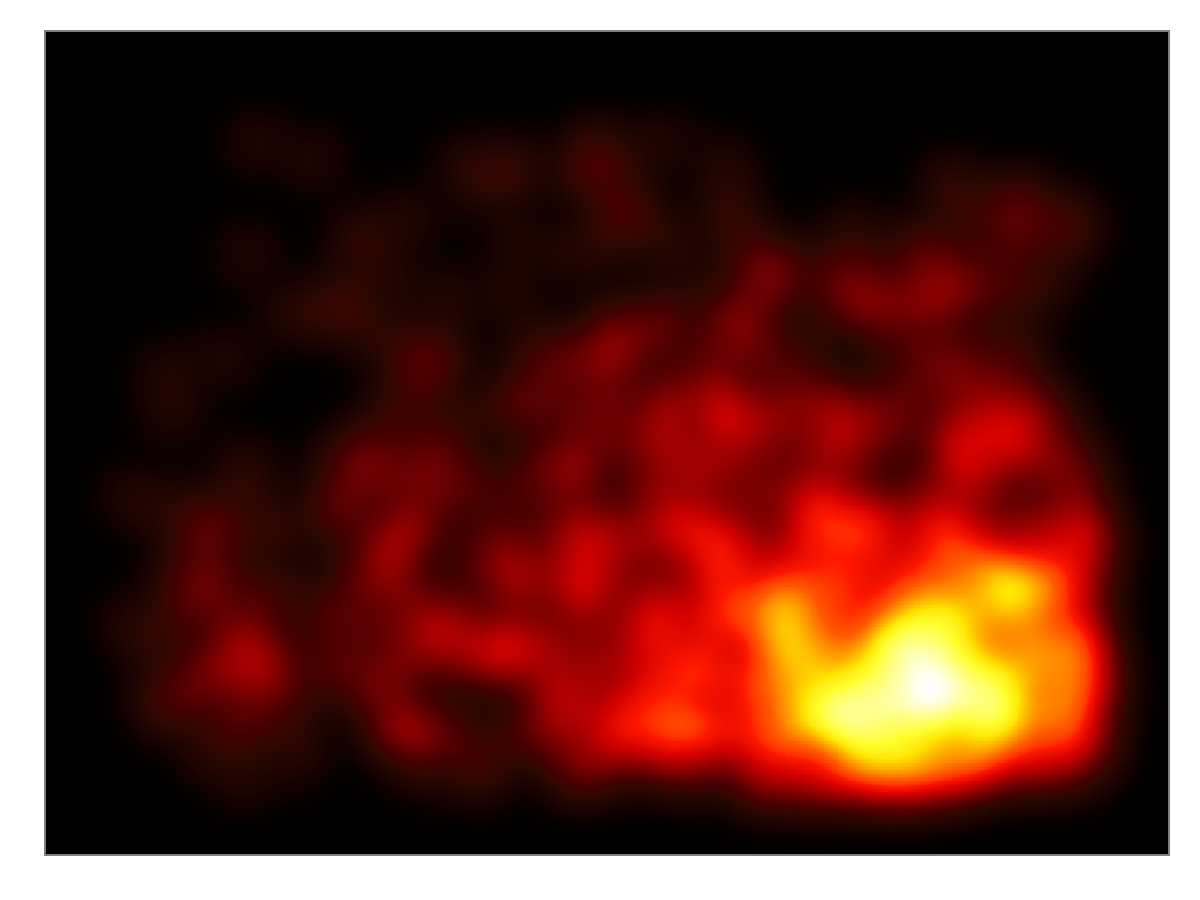
\includegraphics[width=2.5cm]{../scripts/heatmaps/SaccadicFlowMaps/Figures/BBias_33.pdf}}
\caption{Saccade landing positions from fixations that were in different sections of the screen. Data from each plot has been separated into fixations in 9 spatial bins, with the screen being divided into thirds in both horizontal and vertical aspects.}
\label{fig:empiricalSaccadicFlow}
\end{figure}

%%%%%%%%%%%%%%%%%%%%%%%%%%%%%%%%%%%%%%%%%%%%%%%%%%%%%%%%%%%%%
\subsection{The central bias}
%%%%%%%%%%%%%%%%%%%%%%%%%%%%%%%%%%%%%%%%%%%%%%%%%%%%%%%%%%%%%
 
There is a strong tendency for people to look close to the centre of pictures \citep{tatler2007, tatler2005, canosa2003, clarke-tatler2014} and videos \citep{tseng2009,loschky2015} presented on computer screens. There have been a number of suggestions for why this might be, the simplest being that the centre of the stimulus array is the best place to look to make use of parafoveal vision. Another possible explanation for this effect is that the muscles of the eye show a preference for the `straight ahead' position, re-centring in the orbit of the eye socket for most comfortable contraction of the ocular muscles (an \emph{orbital reserve} \citep{fuller1996}). As most scene viewing experimental set-ups stabilise the head to increase the accuracy of the eye tracking, and most scenes are presented in the centre of computer displays, such a re-centring mechanism would mean that the centre of images would indeed be preferentially selected. However, when scenes are scrambled into four quadrants, fixations are located near to the centre of each quadrant, rather than the display centre \citep{stainer2013}, suggesting that the central tendency is responsive to the scene itself rather than to the frame of the monitor upon which the scene is displayed. 

Another possible explanation for the central fixation bias is that it represents a response to \emph{photographer bias} in scenes, as photographers tend to frame their shots to include the most important content in the centre of the scene. However, when \cite{tatler2007} presented scenes where the image features were biased towards the edge of the scene, the central fixation bias persisted. The final possibility is that as a consequence of repeated exposure to photographer bias, the centre of scenes is simply where people are \emph{trained} to look at images \citep{parkhurst2002}. Such learning of spatial probabilities of targets can explain why, for example, people tend to look around the horizon when searching for people in natural scenes \citep{birmingham2009, torralba2006, ehinger2009}. Expecting to find interesting content in the centre of scenes might be a consequence of this hypothesis typically being correct. 

Irrespective of why it occurs, \cite{clarke-tatler2014} showed that the characteristics of the central bias are remarkably consistent across a series of eye movement databases over tasks such as free-viewing, visual search and object naming. They proposed a simple, standardised central baseline based on a multivariate Gaussian, an demonstrated that it outperforms similar measures previously used in the literature.

\subsection{Other Behavioural biases in saccades}
While the central bias has attracted the most attention (at least in terms of models of visual attention), a number of other biases have been documented. These are discussed below. 

\textit{Horizontal Saccades}: Several researchers have noted that when viewing scenes there is a higher proportion of eye movements in horizontal directions than vertical or oblique movements \citep[e.g.][]{gilchrist2006,foulsham2008,tatler2008,lappe1998,lee2002}. There are a number of possibilities as to why this tendency exists. Firstly, there may be a muscular or neural dominance making oculomotor movements in the horizontal directions more likely. Secondly, the characteristics of photographic images may mean that content tends to be arranged horizontally by the photographer. In such situations, horizontal saccades may be the most efficient way to inspect scenes. Thirdly, using horizontal saccades in scene viewing might be a learned strategy. Observers may learn the natural characteristics of scenes based on previous experience, and therefore demonstrate an increased likelihood of moving in the horizontal direction. A final explanation is that this tendency is a consequence of the aspect ratio of visual displays, which normally allow for larger amplitude saccades in the horizontal than vertical directions \citep{wartburg2007}.

Results from Foulsham and colleagues suggest that the outline of the displayed scene has a marked effect on saccade directions during viewing. Indeed, \cite{foulsham2008} found that when the orientation of an image is rotated, the distribution of saccade directions follows the orientation of the scene. Furthermore, when a scene is presented in a circular aperture, the tendency to make horizontal saccades disappears, being replaced by a tendency to make vertical saccades relative to the image orientation \citep{foulsham-kingstone2010}. However, when using fractal images (where images do not have an obvious orientation), observers tend make horizontal saccades, regardless of the angle that the image is presented. These findings suggest that directional biases in saccades are not only influenced by the shape of the displayed scene but also its content.

\textit{Coarse-to-fine}: Another robust pattern in human saccadic behaviour is the tendency to make large eye movements after the initial scene onset, and smaller saccades as the trial unfolds \citep{over2007, pannasch2008,antes1974}. This is often accompanied by an increase in fixation durations,  and is framed as a move from ambient to focal processing \citep{follet2011,velichkovsky2002,unema2005}. \cite{godwin2014} successfully replicated these findings, but they offered an alternative explanation, namely that this behaviours is driven stochastic factors that govern eye movements.


\textit{Leftwards bias}: Several studies have shown that observers exhibit a bias to fixate the left half of a stimulus over the right \citep{ossandon2014,nuthmann-matthias2014,learmonth2015,zelinsky1996, brandt1945}. This effect falls under the more general spatial attention bias of psuedoneglect \citep{bowers-heilman1980}, which also affects tasks such as line bisection. The leftwards bias is typically short-lived, affecting only the first couple of saccades after scene onset, and while it is robust, it is comparatively weak compared to other biases in scene viewing. For example,  \cite{dickinson-intraub2009} found $62\%$ of initial saccades were directed to the left half of the image during free viewing. There is some evidence that this bias is related to native reading direction \citep{friedrich2014}.

\textit{Saccadic Momentum and Inhibition of Return}: Several studies have described sequential dependencies during free viewing that bias saccades to repeat the same vector and amplitude (known as saccadic momentum) and to bias saccades away from returning to previously-visited targets (known as inhibition of return). Although both of these phenomena bias fixations away from previously-fixated locations, they differ in that inhibition of return is bound to a location in the search array, i.e. it is coded in object-based or spatiotopic coordinates (e.g. \cite{krueger-hunt2013}), while saccadic momentum has been characterised as a basic tendency to repeat the same motor program \citep{wang2011}. Inhibition of return, unlike saccadic momentum, is task-dependent \citep{dodd2009} and is disrupted by removing the scene or inhibited object  \citep{klein-macinnes1999, takeda-yagi2000}.  \cite{macinnes2014} observed both of these mechanisms operating during free visual search of a complex scene, but presumably only saccadic momentum would be consistently observed for all tasks and images. 

\subsection{The present study}

These biases, in particular, the central bias, are important to take into account when evaluating the performance of models of fixation location, and investigating relationships between eye movement data and other factors. The main contribution of this manuscript is to introduce the \textit{saccadic flow} model. This can be thought of as a generalisation of the central bias: instead of simply characterising the image-independent probability of fixating $(x_i, y_i)$ we model the conditional probabilities $p(x_i,y_i|x_{i-1}, y_{i-1})$. i.e. the probability of making a saccade from to $(x_i,y_i)$ given we are currently fixating $(x_{i-1}, y_{i-1})$.

In Section \ref{sec:biases} we describe the saccadic flow model and an improved version of the central bias model. The model's ability to account for eye movements during scene viewing is evaluated over 15 previously published datasets. These cover a range of types of images and viewing tasks. In Section \ref{sec:usingbiases} we demonstrate how the central bias and saccadic flow can be used to improve analysis and visualisation methods. In particular, we present bias-weighted gaze landscapes, and demonstrate an interaction between the likelihood of a saccade under different bias models and bottom-up visual salience. Finally, we investigate the short-comings of these generative models by comparing synthesised data to human eye movements. 